\documentclass[12pt]{report}                  % Times New Roman, 12pt
% \usepackage{gscale_thesis_singlespace} % Single spaced thesis
\usepackage{gscale_thesis_doublespace} % Double spaced thesis
\usepackage{fancyheadings}                   % Header and footer styling
\usepackage{natbib}                               % Bibliography formatting
\usepackage{setspace}                           % Allows double spacing but skips headers/footers
\title{Assurance for Machine Learning systems}
\halftitle{Assurance for Machine Learning systems} % 60 Characters Max. Including Spaces

\author{Milad Hassani}
\shortauthor{M. Hassani} % Used for page header

\dept{computing and software} % The department you are part of; Must be all lower case
\field{Computer Science} % What field your thesis is in

\prevdegreeone{Ph.D. (Computer Science),\\ McMaster University, Hamilton, Canada}
\prevdegreetwo{Ph.D.} % Just your degree's field

\submitdate{June 2021}
\copyrightyear{2021}

\principaladviser{Dr. Richard Paige} % Your Supervisor
                                % LaTeX variables for preface pages/headers
\setcounter{tocdepth}{1}                        % Limits the TOC to chapter and section names

% Additional packages
\usepackage{graphicx}                                   % Allows the inclusion of figures
\usepackage{subcaption}                               % Allows captions to be added to subfigures
\usepackage[justification=centering]{caption}       % Centers caption text
\usepackage[hidelinks]{hyperref}                    % Linking to labels and external URLs
\usepackage{array}                                        % Used for table formatting
\newcolumntype{P}[1]{>{\raggedright\let\newline\\\arraybackslash\hspace{0pt}}m{#1}}
\usepackage{booktabs}                                 % Fancy-style tables
\usepackage{longtable}                                 % Allows for tables that are more than one page long
\usepackage{float}                                         % Better figure placement control
\usepackage{enumerate}   
\usepackage[shortlabels]{enumitem}                            % Numbered lists 
\usepackage[shortcuts]{extdash}                  % Allows manual hyphenation of hyphenated words
\usepackage{amsmath}                                % Non-standard math symbols
\usepackage{amsfonts}                                % Extended fonts for 
%mathematics
\usepackage{xcolor}
\usepackage{csquotes}                            % Allows quotes
\usepackage{multirow}
\usepackage{url}
\numberwithin{equation}{section}                 % Numbers equations based on their section

% ********************************
\begin{document}
\beforepreface                                         % Half title page, title page, declaration page   
%   \prefacesection{Lay Abstract}

A lay abstract of not more 150 words must be included explaining the key goals and contributions of the thesis in lay terms that is accessible to the general public.                                  % Lay Abstract
  % \subimport{../main/}{library.bib}
% \bibliographystyle{plain}
% \bibliography{library.bib}

\prefacesection{Abstract}

According to Software maintenance consumes 75\% of the total IT budget of a company \cite{cisq_report}.

According to Curtis \cite{cisq_report}, in 2018, number of software failures had surpassed 100M which consequently represent a significant waste of resources. 
                                      % Abstract
  %%\thispagestyle{empty}
\null\vfill
\begin{center}
%\textbf{Dedications}
%\linebreak
\textsl{Your Dedication \\ Optional second line}
\end{center}
\vfill
                                      % Dedication
  %\prefacesection{Acknowledgements}

Acknowledgements go here.                 % Acknowledgements
  \referencepageswithnotations{notation} % Table of Contents, List of Figures, List of Tables, Notations
  %\referencepages                                 % No notations version (choose one)
\afterpreface                      
  
  
  \chapter{Introduction}

\section{Benefits of Architecture Recovery}
\begin{itemize}
    \item New members of a development team can benefit from the architecture by having access to the group memory of all the artifacts generated during the development process. Tools such as Hipikat \cite{Cubranic2005} can generate such a memory by analyzing which developers have the most contribution for a component. Leveraging this information, new developers will know which team member to contact in case of any questions.
    \item Project managers can benefit from the information on which parts of the project is actively changing and how this change is affecting the structure of the project \cite{leh80}.
    \item By creating a mapping between the changes and author identifiers, project managers can also understand who has worked on an artifact and thus, is more knowledgeable about a problem at hand for the same artifact \cite{Girba05}.
    \item Identify the distance between the requirement and implementation of the system, i.e., as-is-architecture and as-it-should-be architecture \cite{eixelberger98}
    \item Architecture Recovery can help learn the structure of a program and how it satisfies the domain needs 
\end{itemize}

% Why not? \cite{svetinovic18}
% \begin{itemize}
%     \item Most developers like to concentrate exclusively on programming.
%     \item Design documents are almost never in synchronization with code.
%     \item During active development, lot of time is spent updating design documents.
%     \item The produced documents are not used much by programmers.
%     \item Tool support for roundtrip engineering is not good enough.
% \end{itemize}

% \section{To read list}
% \begin{itemize}
%     \item Architecture  description  language  (ADL) or Architecture Structure Description Language (ASDL).
%     \item Configuration management (CM) systems [Burrows and Wesley 2001]
%     \item 
% \end{itemize}
                  
        \setcounter{figure}{0}
        \setcounter{equation}{0}
        \setcounter{table}{0}
        
  \chapter{Machine Learning}
\label{chap:ML}

In this chapter we will start by reviewing definitions of ML in the literature, and continue with definitions of learning categories such as supervised, unsupervised and reinforcement learning. Next, we explore how data is managed in a given ML problem, as this is relevant to safety, certification and assurance (for example, data might form some of the evidence used in an assurance case). Finally, we review how performance of ML methods is measured.

\section{Definition}
Machine learning algorithms can extract patterns and learn from data \cite{IanGoodfellow2016}. A brief definition of learning can be given as \cite{mitchell1997machine}
\begin{displayquote}[][]
    "A computer program is said to learn from experience \textit{E} with respect to some class of tasks \textit{T} and performance measure \textit{P}, if its performance at tasks in \textit{T}, as measured by \textit{P}, improves with experience \textit{E}."
\end{displayquote}

A task is the main objective of using an ML algorithm. For example, in an autonomous vehicle, driving the car is the task. A task is not the process of learning. Learning is used as a means to achieve an ability to accomplish a task \cite{IanGoodfellow2016}. With developments in ML methods, they have been applied to different tasks, some examples of tasks are classification, regression, transcription, machine translation, denoising \cite{IanGoodfellow2016}.

The performance measure is used to quantify how successfully a task is accomplished, equivalently, number of erroneous outputs could be used as a way of indicating a method's performance. 

Based on the above-stated definition, the ML algorithm undergoes an experience in the process of learning. This experience is generally classified into \textbf{unsupervised}, \textbf{supervised} and \textbf{reinforcement} learning.

\section{Learning types}

Unsupervised learning finds the properties of the overall structure of the dataset. Clustering as an example of unsupervised learning, finds clusters within a dataset and assigns each data-point to one of them.\\In supervised learning, on the other hand, data-points that the learning algorithm experiences have a label. This label acts as a guide for the ML algorithm. The term supervised arises from the fact that the labels instruct the algorithm what to do. Labels are unavailable in unsupervised learning and the ML system is responsible to make sense of the data independently \cite{IanGoodfellow2016}. 

Reinforcement learning (RL) algorithms experience an environment instead of a fixed dataset. The algorithm should learn how to maximize a reward function by taking an appropriate action \cite{sutton1992introduction}. The learner discovers this appropriate action by trying different actions and observing the value of the reward function. Actions not only affect the immediate reward, but can also change next actions' rewards. Trial and error search and delayed reward are two main characteristics of RL.\\The learner, also known as the agent in RL terms, should have the capability to sense the state of the environment, take actions that can alter the state and also have a goal to reach by taking actions. These three aspects are included in the reward function used by the agent \cite{sutton1992introduction}. 

\section{Data in ML}

Evidently, ML algorithms need data to learn and function. A dataset can be described as a \textbf{design matrix}. Every row in the matrix contains an example, also known as data-point, and each column is a feature. Iris dataset is one of the first ones used in statistics and ML \cite{Fischer1936Iris}. This dataset is comprised of 150 examples which have 4 features each. One example corresponds to one individual plant. Sepal length, sepal width, petal length and petal width are recorded as features of each plant \cite{Fischer1936Iris}.
This means that if $X$ is the matrix, we can say $\mathbf{X} \in R^{150 \times 4}$

The ML model will ultimately be deployed and used in a real world situation, hence, we are interested in how well an ML model performs on the data it has not seen before, this is also known as \textbf{generalization}. A portion of dataset is therefore not used in the training process and reserved as a \textbf{test set}. The data used in the training process is accordingly referred to as the \textbf{training set} \cite{IanGoodfellow2016}. 

In some cases, the training and test datasets might be limited in size and to have a better generalization, it is necessary to use as much of the data for training as possible. In other words, there will be less data available to estimate the performance of the model. One solution for this situation is \textbf{cross-validation}. The entire dataset is split into ${S}$ subsets. In each run, ${S - 1}$ subsets are used for training and one remaining subset is the test set. For the next run, a different test set is selected \cite{bishop2006pattern}. Figure \ref{fig:crossv} shows selection of subset for ${S = 4}$.

\begin{figure}
    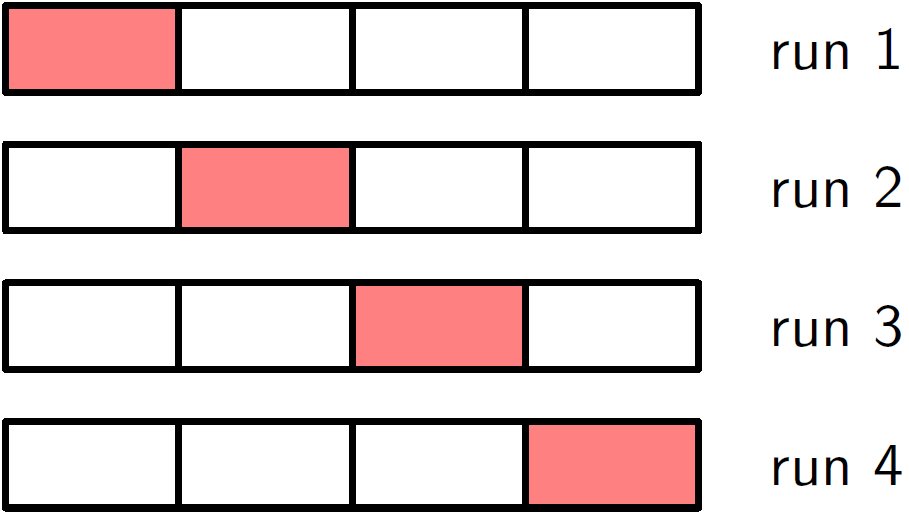
\includegraphics[width=0.5\linewidth ]{figures/crossv.png}
    \centering
    \caption{Cross validation for S=4 \cite{bishop2006pattern}.}
    \label{fig:crossv}
\end{figure}


\section{Performance measures}
In classification tasks, \textit{confusion matrix} is a way to demonstrate differences between predicted and true classes \cite{Bradley1997}. Table \ref{tab:conf-mat} shows the structure of a confusion matrix.
% Please add the following required packages to your document preamble:
% \usepackage{multirow}
\begin{table}[]
    \centering
    \begin{tabular}{llccll}
                                &    & \multicolumn{2}{l}{Predicted Class} &    &  \\ \cline{3-4}
                                &    & C-               & C+               &    &  \\ \hline
    \multirow{2}{*}{True class} & C- & Tn               & Fp               & Cn &  \\
                                & C+ & Fn               & Tp               & Cp &  \\
                                &    & Rn               & Rp               & N  &  \\ \hline
    \end{tabular}
    \caption{A confusion matrix}
    \label{tab:conf-mat}
\end{table}

In Table \ref{tab:conf-mat} \textit{Tp} and \textit{Tn} represent true positives and true negatives respectively. \textit{Fp} and \textit{Fn} are in the same manner the count of false positives and false negatives respectively. \textit{Cp} and \textit{Cn}, therefore, are the total number of positive and negative examples. Finally, \textit{Rp} and \textit{Rn} denote total number of predicted positives and negatives, respectively \cite{Bradley1997}.

A variety of performance measures can be calculated from the confusion matrix, e.g., accuracy, precision, sensitivity and specificity \cite{Bradley1997}. Accuracy is often considered as a performance criteria which is simply the fraction of correctly classified samples to total samples, i.e., {\large $\frac{Tp + Tn}{N}$}. It is also possible to obtain the same information by calculating the \textit{error rate}.

The Receiver Operating Characteristic (ROC) curve helps to find a pareto-optimal point between true and false positive rates as the decision threshold changes \cite{Bradley1997}. Each point on the curve represents the Tp (vertical axis) and Fp (horizontal axis) for a decision threshold. The area under ROC curve (AUC) is, therefore, a measure of the sensitivity of the model to changes in operating conditions. If AUC value is at maximum, i.e., one, it can be concluded that the $P(Fp) = 0$ and $P(Tp) = 1$ even when the operating conditions change.

According to the mandates of the ML application, various performance metrics can be calculated from the confusion matrix, \cite{Sokolva2008} introduces twenty four of these metrics and in which applications they can be used.
% \subsection{Loss function}
% In some cases, the impact of misclassification is not the same for each class. For example, if a patient without cancer is classified as a cancer patient, there will be mental distress. However, if a cancer patient is diagnosed as healthy, the results could be premature death. A loss function is defined to penalize the second type of mis-classifications even if it is with the cost of having more errors in the other class \cite{bishop2006pattern}.\\
% \textcolor{red}{incomplete - add where else loss functions are used}
% \textcolor{green}{include it in the NN section}
% \subsection{No free lunch theorem}
\section{Neural networks}
In this section we briefly review the structure of neural networks and their building blocks. As the name suggests, neural networks are fundamentally a collection of entities called \textit{neurons}, which can hold small units of data. Here we consider a simple neural network, depicted in Figure \ref{fig:nn}, consisting of a hidden layer and an output layer. Hidden layers are the ones not directly accessible from the outside world, i.e., not the input or output layers.
\begin{figure}
    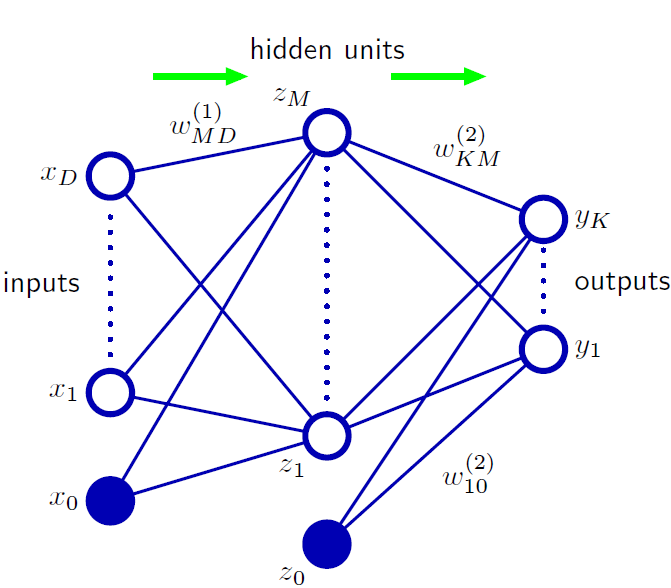
\includegraphics[width=0.5\linewidth ]{figures/neural_net.png}
    \centering
    \caption{Structure of a two layer neural network. \cite{bishop2006pattern}.}
    \label{fig:nn}
\end{figure}

Using the notation in \cite{bishop2006pattern}, if we have $D$ input variables, $x_{i}$, we can calculate linear combinations $a_{j}$ such that
\[
    a_{j}=\sum_{i=1}^{D}w^{(1)}_{ji}x_{i} + w^{(1)}_{j0}
\]
Here, $1 \leq j \leq M$ where $M$ represents number of neurons (nodes) in the hidden layer. The superscript $(1)$ corresponds to the first layer of the network, i.e., the hidden layer in this example. $w^{(1)}_{ji}$ are called weights and $w^{(1)}_{j0}$ are biases for the hidden layer.
The $a_{j}$ values are referred to as \textit{activations}. Next, we use activation function, $h$, to calculate $z_{j}$, such that
\[
    z_{j}=h(a_{j})
\]
The activation function is required to be differentiable due to the differentiation in the learning process. $z_{j}$ values are then used to compute the linear combinations $a_{k}$ in a similar manner to the previous layer, i.e., 
\[
a_{k}=\sum_{j=1}^{M}w^{(2)}_{kj}z_{j} + w^{(2)}_{k0}
\]
$a_{k}$ is the output layer activation, therefore, similar to the hidden layer, an activation function, $\sigma$, will be used to reach final output values of the network, $y_{k}$.
\[
y_{k}=\sigma(a_{k})
\]
Substituting values from all layers the final $y_k$ will be

\[
y_{k}(x,w)=\sigma\bigg(\sum_{j=0}^{M}w^{(2)}_{kj}h \bigg( \sum_{i=0}^{D}w_{ji}^{(1)}x_i \bigg)\bigg)
\]
% \textcolor{red}{Should I include the training process for neural networks? It takes more space. At least 1-1.5 pages.}


\section{Trends in ML research}
With the rapid development of frameworks and libraries in ML, it is increasingly straightforward to apply ML algorithms and tools in different applications. It is possible to develop smaller models which in turn makes applications such as IoT \cite{iot_apps_conf} more feasible. 
Prevalence of ML raises important questions in its fairness \cite{FairML2018}, privacy \cite{Federated2019}, and safety \cite{Varshney2017}. The term \textit{responsible ML} covers the social impacts of using ML in everyday life.
Moreover, the desire to have faster, better performing ML systems has lead to areas such as quantum ML \cite{QuantumML2017}. As a matter of fact, quantum ML has been one of the initial motivations for experiments which lead to the famous quantum supremacy \cite{Quantum_sup}.                  
       \setcounter{figure}{0}
       \setcounter{equation}{0}
       \setcounter{table}{0}

  \chapter{Safety and assurance}
\label{chap:safety}

In this chapter, we start with a basic definition of safety to set the context. Next, we delve into (safety) assurance cases and how they are structured. Finally, we review a representation method for assurance cases called Goal Structuring Notation (GSN).

\section{Definitions}
\subsection{Safety}

Safety is defined in ISO 26262 \cite{organization2018iso} as:
\begin{quotation}
Absence of unreasonable risk.
\end{quotation}  
An unreasonable risk is a \cite{organization2018iso}:
\begin{quotation}
Risk judged to be unacceptable in a certain context according to valid societal moral concepts.
\end{quotation}
Various safety standards have been developed for different industries and activities. Some examples are ISO 26262 for functional safety of road vehicles, DO-178C for aerospace industry, ISO 8124 for safety of toys, ISO 7164 for healthcare organization management.

\subsection{Assurance}
Assurance is defined in ISO 15026 to be \cite{iso15026-1-2019}
\begin{quotation}
Grounds for justified confidence that a claim has been or will be achieved.
\end{quotation}
Assurance is, therefore, the grounds on which the users of a system can rely on its functionality. It is specially important for systems with complexity, such as ML, to give assurance to the users before they start utilization. The level of this assurance is closely related to the level of dependence or trust needed from the users' side. Adequate evidence and arguments need to be present to justify the safety and reliability of the system. The basis for this justification is achieved with reducing uncertainty in measurements, observations, estimations, predictions, information, inferences or effects of unknowns \cite{iso15026-1-2019}. 
\section{Safety Assurance Case}
Assurance cases have been successfully used in various industries to specify an argument as to why a system can be safely used for a specific application in a specific context \cite{Ashmore2021}.
A recent definition of safety assurance case is described in \cite{Bloomfield2010} as


\begin{displayquote}[][]
"A structured argument, supported by a body of evidence, that provides a compelling, comprehensible and valid case that a system is safe for a given application in a given environment"
\end{displayquote}
A structured argument is a \cite{Omg2010}
\begin{displayquote}[][]
"connected series of statements or reasons intended to establish a position...; a process of reasoning."
\end{displayquote}
Reasons used in a structured argument can be considered as premises in logical terms and a conclusion can be drawn based on them \cite{Omg2010}.  
% A safety assurance case \textcolor{red}{(Assurance case in short)} justifies safety of a system by bringing a valid argument that a set of claims are justified, given that a set of assumptions are fulfilled \cite{Burton}.
The purpose of using an assurance case is to communicate a clear, comprehensive, defensible argument that a system is safe to be used in a particular context \cite{gsn2004Kelly}. Assurance cases are comprised of five basic components: claims, arguments, evidence, justifications and assumptions. The most common use of assurance cases is to give assurance about system's functionality and properties to the parties which were not involved in the process of developing the system \cite{iso15026-1-2019}.

Assurance cases are used to explicate and support reasoning, albeit in a subjective manner, especially when compared to the logical proofs which consider an absolute truth. In other words, assurance cases are useful because the full range of a system's properties are not always representable in a logical formalization. Also, assurance cases may sometimes be disproved because the underlying logical theory used in them is not relevant \cite{iso15026-1-2019}.

Since assurance cases are considered artefacts, they inherit quality related properties of them such as: the structure of its content, semantic features such as completeness, creation and maintenance. The conclusions of the assurance case should also be stated clearly with clear level of uncertainty \cite{iso15026-1-2019}. 
% \textcolor{red}{more from 15020 about assurance cases?}

\section{Goal Structuring Notation}
When the safety assurance case is more complex in nature, textual representation suffers to express the case in a clear and understandable way. Figure \ref{fig:text-case} shows an example of such problem where the English structure of the argument is hard to understand. Having multiple cross references is specially difficult to capture in text \cite{gsn2004Kelly}.
\begin{figure}
    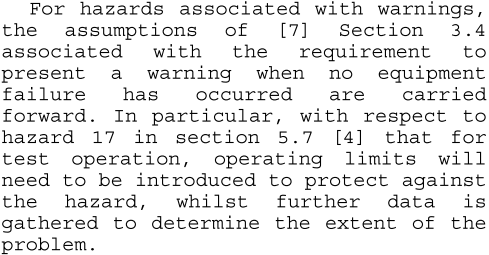
\includegraphics[width=0.5\linewidth ]{figures/textual_case.png}
    \centering
    \caption{Problems associated with textual representation \cite{gsn2004Kelly}.}
    \label{fig:text-case}
\end{figure}

The Goal Structuring Notation (GSN) is a graphical notation for safety argumentation. A GSN specification explicitly represents elements of a safety argument and the relationships among these components. For example, how requirements are supported by claims or how claims are supported by evidence or how the case has a defined context \cite{gsn2004Kelly}. Figure \ref{fig:gsn} depicts basic building blocks of a GSN with example instances of each element. 

\begin{figure}
    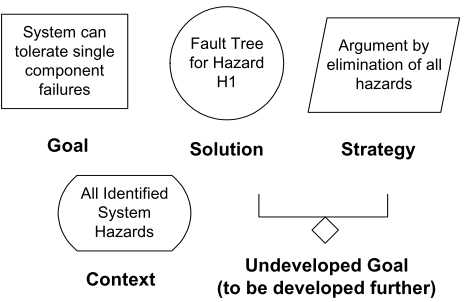
\includegraphics[width=0.5\linewidth ]{figures/gsn.png}
    \centering
    \caption{Basic elements of a GSN \cite{gsn2004Kelly}.}
    \label{fig:gsn}
\end{figure}

\section{An example of GSN}

The goal structure is used to show how goals (claims about the system) can be split into sub-goals successively until the sub-goal can be directly supported by available evidence. Figure \ref{fig:gsn-example} represents an example of a GSN.

\begin{figure}
    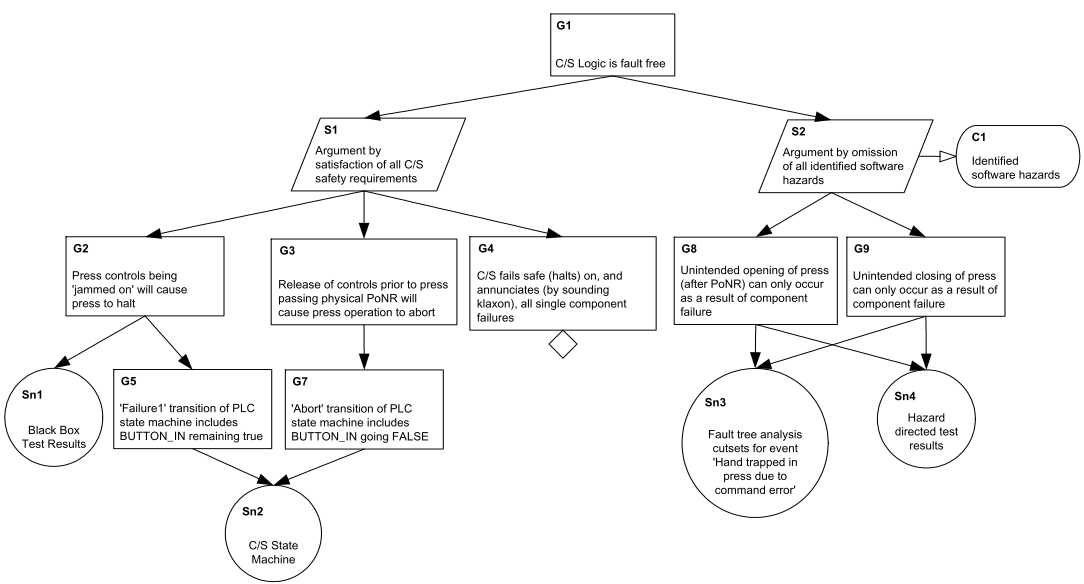
\includegraphics[width=0.9\linewidth ]{figures/gsn-example.png}
    \centering
    \caption{An example of a goal structure \cite{gsn2004Kelly}.}
    \label{fig:gsn-example}
\end{figure}

In this example, "Control System (C/S) logic is fault free." is one single top level goal. The main goal is then divided to two sub-goals through strategies $S1$ and $S2$. These two strategies are then supported by five sub-goals $G2-G4$ and $G8-G9$. In a goal structure, there will be a stage where the sub-goals can be directly supported by solutions. In this example, sub-goals $G8-G9$ are supported by $Sn3-Sn4$ and there is no need to break down the goals further in this branch \cite{gsn2004Kelly}.\\

% \textcolor{red}{write about CAE(Claims Arguments Evidence)}

\section{Trends in safety research}
Safety assurance should constantly evolve and adapt to the new paradigms in industry. With advent of Industry 4.0, new risks and challengers arise in workspace and occupational safety. Safety 4.0 is a response to these new challenges \cite{Laciok2021}. There is a growing number of research projects on using the recent advances in ML technologies to enhance safety, some of which is referred to as "safety informatics \cite{Wang2019}". In addition, 5G technology has raised concerns about the long term health consequences. Critiques are collecting evidence that 5G may result in skin cancer and the millimeter wave radiation can ultimately affect the nervous system \cite{Russel2018}. Unmanned Aerial Vehicles (UAV), or commonly known as drones, are rapidly spreading in industrial usage and thus their safety and privacy challenges are of interest \cite{Aydin2019}.                  
       \setcounter{figure}{0}
       \setcounter{equation}{0}
       \setcounter{table}{0}

  \chapter{Literature Review}
\label{chap:literature}

In this chapter we will briefly review some of the literature about the safety of ML methods and identify major research questions in this area. 
Today, ML is used in variety of applications with varying safety requirements. This diverse portfolio includes smart phones \cite{smartphone2012}, cars \cite{Levinson2011}, surgical equipment \cite{Egert2020}, construction industry \cite{bilal2020} and many more. A fault in an ML system, e.g. a misclassification, has different repercussions in each application. An out of focus image taken by a camera can be easily remedied, but a malfunction in a surgical equipment could be fatal and result in an irreversible situation. Therefore, assuring safety is an essential part of the design process for these applications.

One major issue in safety assurance for ML is guaranteeing that the training data is complete and relevant. Data used in the operational stage is by definition relevant, however, training data may not reflect all possible situations that the learning algorithm needs to be exposed to. On the other hand, the operational environment may change and the training data may diminish in relevancy. As discussed in detail later in this chapter, assuring completeness and relevancy is challenging and may not always be feasible. 

% \textcolor{blue}{IDEA: Creating a map of ML. Listing all successful applicaitons of ML in industry for example.}
% 
% \textcolor{red}{As this part is mostly concerned with RL I should put it in a separate subsection}
In \cite{Amodei2016}, five major research problems associated with unsafe behavior of ML models is presented. They can be summarized as
\begin{enumerate}
	\item Avoiding Negative Side Effects: How to ensure that the model will not disturb the environment while pursuing its goals, e.g. can a cleaning robot knock over a vase because it can clean faster by doing so? Can we do this without manually specifying everything the robot should not disturb.
	
	\item Avoiding Reward Hacking: How to ensure that the model does not avoid situations to achieve a higher reward. For example, if we reward the robot for achieving an environment free of messes, it might disable its vision so that it won’t find any messes, or cover over messes with materials it can’t see through, or simply hide when humans are around so they can’t tell it about new types of messes.
	
	\item Scalable Oversight: How to ensure the model respects the parts of the objective function that are expensive to evaluate and makes a safe approximation of these parts. 
	For example, in the cleaning robot example, if the user is happy with the cleaning quality is an expensive objective function, but it can be approximated to presence of any dirt on the floor when the user arrives.
	
	\item Safe Exploration: How to ensure that the ML model explorations are safe. For example, the robot should experiment with mopping strategies, but putting a wet mop in an electrical outlet is a very bad idea.
	
	\item Robustness to Distributional Shift: How to ensure that the model performs robustly if the environment shifts from the training environment. For example, strategies a cleaning robot learns for cleaning an office might be dangerous on a factory work-floor.

\end{enumerate}

% Some of the above 
\section{Machine Learning lifecycle}

To obtain assurance for ML systems it is essential to understand the ML lifecycle and how to analyze safety in each step. In this section we will first introduce these steps and review some of the safety measures for each step. This lifecycle follows a spiral process model, i.e., the stages are iteratively repeated to actively reduce risk \cite{Boehm2000}. ML lifecycle is comprised of four stages \cite{Ashmore2021} 

\subsection{Data Management}
\label{sub:DM}
This stage involves collecting, preprocessing, augmenting and initial analysis of data. The training and validation datasets are also prepared in this step.
From assurance perspective, the data collected in this step should be
\begin{itemize}
    \item Relevant: The dataset should be relevant to the desired functionality of the final model. For example a dataset of handwritten letters in Japanese language cannot be used for English language. In many cases, a pre-existing dataset will be used to train the model. This dataset should be obtained from trusted sources with an encrypted transmission medium. An attacker can add irrelevant samples into the training dataset to make the final model behave in a specified way for particular inputs \cite{Chen2017}. The irrelevant data injected in the dataset is called a backdoor \cite{Chen2017} Despite early efforts in detecting backdoors in face recognition \cite{Wang2019} finding a general solution is still an open challenge.
    \item Complete: The features of a dataset should not have unintended correlations that can confuse the classifier. For example, if a classifier is trained on pictures of wolves and huskies, and all wolves have snow in the background, it may be concluded that snow in the background means a wolf \cite{Ribeiro2016}. In this case the dataset is not complete because it does not include pictures of wolves with different backgrounds. Exploratory Data Analysis (EDA), is an important step in examining completeness of a dataset. It is also important to identify how the data points are distributed in the input sample space, measures such as gap ratio \cite{Teramoto} can be used to evaluate uniformity. To further increase completeness of the dataset, Generative Adversarial Networks (GAN)s can be used to learn the distribution of the classes and generate more data \cite{Antonio2018}. 
    \item Balanced: For classification problems, it can happen that one class has significantly more data-points in the training set than the others and thus, classifier has more exposure to that class. In addition, imbalance can also happen in features, for example, if age is one of the features and data is collected from primary schools in a city, an imbalance in age feature is expected. The impact of feature imbalance on final models' behavior is an open challenge.
    \item Accurate: This property considers factors like sensor accuracy, correctness of data collection and processing method. In the case of supervised learning, labels' accuracy is important. In many applications it is needed to manually label data. Various crowdsourcing platforms is developed for this purpose however, accuracy of the labels is debatable and should be investigated subsequently \cite{Sheng2019}. The data collection process should be documented to identify potential inaccuracies \cite{Ashmore2021}.
\end{itemize} 

\subsection{Model Learning}
In this stage of the ML lifecycle, the type of the model and its hyper-parameters are selected. For some ML applications, the dataset is very large or the model structure is complex and therefore, the learning process needs considerable amount of computational power. In these cases, it is reasonable to take advantage of a previously trained model and adapt it to our needs by re-training only the parts that are different from the other application. This process is called \textit{transfer learning} \cite{IanGoodfellow2016}. If there is a need to do transfer learning, it will be decided at this stage and finally the learning process starts using the train dataset obtained in previous stage.
In order to have a clear view of the model in safety related aspects, the final model should be \cite{Ashmore2021}  
\begin{itemize}
    \item Performant: As a requirement for a safer model, it should have a justifiable performance according to the measures introduced in Chapter \ref{chap:ML}. Judging model's performance solely on one composite metric, is sometimes inaccurate and not contextually relevant \cite{Flach2019}. While measures such as accuracy represent a general idea of model's performance by averaging over all outputs, they lack information on outcomes for a specific example. Intuitive Certainty Measure (ICM) provides an estimate of model's performance for a specific example, based on the errors it made in the past \cite{Wang2019}.
    \item Robust: The model should be able to perform as well on the unseen data as the training data, i.e., generalizes well to be considered robust. One solution to increase robustness of the model is to enhance completeness of the dataset, therefore, data augmentation data augmentation is one of the techniques to increase generalization \cite{Ko2015}. GANs as discussed in Data Management section help in completeness of the dataset and, consequently, increasing models' robustness \cite{Antonio2018}.
    \item Reusable: Using transfer learning can help to use the assurance evidence of the original model, provided that the transfer learning is performed in the right context for the source and destination models. However, reusing models comes with the risk that safety issues propagates to the destination model too \cite{Gu2019}. Models trained on popular standard datasets can be found in model zoos such as \cite{zoo21}\cite{zoo-caffe-21}.
    \item Interpretable: This property shows how much the decisions made by the model are explainable and thus helps to analyze the safety of such decisions. Natural language explanations \cite{Krenin2016}, model visualization \cite{Mahendran2015}, explaining by example \cite{Adhikari2018}
\end{itemize}

\subsection{Model Verification and Validation} 
The black swan problem expounds one of the major challenges in validating ML models. A system or a person could incorrectly conclude from abundance of training data samples that common observations are true \cite{koopman2016challenges}. A model which has only seen white swans, may infer that all swans are white and ignore the fact that there are black swans \cite{taleb2007the}. One major challenge is thus making sure that the model works well, i.e., satisfies its requirements, on the data it has not seen before which is also known as generalization. If the model fails in this stage, the process will go back to Data Management or Model Learning steps. Model verification involves requirements encoding, test-based verification and formal verification. The verification stage should be \cite{Ashmore2021}
\begin{itemize}
    \item Comprehensive: Model verification should ensure that all the requirements of the system and also intended goals of the previous stages of ML lifecycle, i.e., data management and model learning, are covered.
    \item Contextually relevant: Verification process should be relevant to the intended use of the ML model. For example an ML model used in autonomous vehicles, we are more concerned about how changes in the environment will affect model's performance and thus, how robust is the model with changes in weather rather than the changes in image quality. 
    \item Comprehensible: Verification results should be understandable for the users. Requirement violations should be clearly expressed in such a way that the cause of it can be identified and fixed \cite{Ashmore2021}. Ideally, the results should also include any black swan biases present in the model \cite{koopman2016challenges}.
\end{itemize}

\subsection{Model Deployment} 
Preparing the ML model to be used in the final application. Activities in stage includes integration, monitoring and updating. To assure safety of this stage of ML lifecycle, the ML model should have the following properties

\begin{itemize}
    \item Fit-for-Purpose: The difference in hardware can cause performance differences between ML stages. Also, each distinct hardware setting where a model is deployed can affect model's performance. For a model to be fit for purpose, the performance seen in the previous stages should be carried over to the deployment phase. 
    \item Tolerable: The system should be able to tolerate occasional incorrect outputs of the ML model. To accommodate this, the host system should be able to identify the incorrect outputs and to replace them with a safe value so that the system continues the normal processing activities.
    \item Adaptable: Deployed models are in many cases needed to be updated due to variety of reasons including operational, legislative or environmental changes. This property indicates how safe is the process of updating. 
\end{itemize}

\section{Open challenges in ML assurance}
Using an ML component in a system poses several challenges in each step of the ML lifecycle. In the data management step, further research is needed to guarantee security of data and its fitness for the purpose. Although a vast amount of research has been conducted in the model learning stage, there is still a need to further study hyper-parameter selection. In addition, with recent successes in transfer learning, there is still need for more research in assuring safety in this area. Furthermore, safety assurance requires ML models to be reusable and interpretable. Model verification assurance is mainly accomplished using test-based and verifications. However, there is still a need to develop methods to encode model requirements into proper and formal tests. In model deployment stage, there is no explicit equivalent for updating models in software engineering world, therefore, there is a need to devise assurance methods for adaptable safety-critical systems \cite{Ashmore2021}.

In some applications requirements for a safe ML system reinforce each other. For example, accuracy in data management stage will most likely result in more performant model. However, in some cases, there is a trade-off between requirements, an explainable model is probably more exposable to cyberattacks \cite{Ashmore2021}. In spite of attempts to address this issue \cite{Johnson2019}, more research is required to adapt these concepts to ML.                    
       \setcounter{figure}{0}
       \setcounter{equation}{0}
       \setcounter{table}{0}

  \chapter{Conclusion}

In this report we first started with the basic definitions and principals of machine learning and safety assurance concept and explored some of the fundamentals in both areas in Chapter \ref{chap:ML} and Chapter \ref{chap:safety} we also glanced currently trending research in these areas. Finally, in Chapter \ref{chap:literature} we reviewed some of the literature in assurance of ML systems and some of the open challenges and research questions in each step of ML lifecycle. Despite significant research into some stages of ML lifecycle, more research is needed in other parts. For example, explainable models, there are no global methods providing insights into complex ML models.  % \textcolor{red}{State some of the major open challenges I found,}
        \setcounter{figure}{0}
        \setcounter{equation}{0}
        \setcounter{table}{0}

% \begin{appendix}
% 	\chapter{Your Appendix}
\label{appendix_a}

Your appendix goes here.

% 		\setcounter{figure}{0}
% 		\setcounter{equation}{0}
% 		\setcounter{table}{0}
		
% 	\chapter{Long Tables}
\label{appendix_b}

This appendix demonstrates the use of a long table that spans multiple pages.

\begin{center}
\begin{longtable}{P{3cm}P{3cm}P{2.5cm}P{3.5cm}}
\toprule
\hline
\textbf{Col A} & \textbf{Col B} & \textbf{Col C} & \textbf{Col D} \\ \midrule

\endfirsthead
\multicolumn{4}{c}{\textit{Continued from previous page}} \\ \hline
\textbf{Col A} & \textbf{Col B} & \textbf{Col C} & \textbf{Col D} \\ \hline
\endhead
\hline \multicolumn{4}{r}{\textit{Continued on the next page}} \\
\endfoot
\hline
\endlastfoot

A & B & C & D \\ \midrule

A & B & C & D \\ \midrule

A & B & C & D \\ \midrule

A & B & C & D \\ \midrule

A & B & C & D \\ \midrule

A & B & C & D \\ \midrule

A & B & C & D \\ \midrule

A & B & C & D \\ \midrule

A & B & C & D \\ \midrule

A & B & C & D \\ \midrule

A & B & C & D \\ \midrule

A & B & C & D \\ \midrule

A & B & C & D \\ \midrule

A & B & C & D \\ \midrule

A & B & C & D \\ \midrule

A & B & C & D \\ \midrule

A & B & C & D \\ \midrule

A & B & C & D \\ \midrule

A & B & C & D \\ \midrule

A & B & C & D \\ \midrule

\hline
\end{longtable}
\end{center}

% 		\setcounter{figure}{0}
% 		\setcounter{equation}{0}
% 		\setcounter{table}{0}
% \end{appendix}

% The bibliography is set up to allow for multiple bib files
\bibliographystyle{plain}
\bibliography{library.bib}

\label{NumDocumentPages}

\end{document}
% ********************************
